\chapter{Testing}

\section{Configurazione dell'ambiente indoor}
La configurazione dell'ambiente consiste nella disposizione dei dispositivi Bluetooth nel modo corretto.
Per poter avere un ricezione dei segnali inviati dagli iBeacon senza troppi disturbi, questi devono essere così disposti:
\begin{itemize}
	\item su pareti regolari a circa 1 metro da terra;
	
	\item lontano da apparecchi che emettono onde elettromagnetiche (ad esempio router wifi);
	
	\item al sicuro da raffiche di vento;
	
	\item in aree in cui non si frappongano oggetti o persone tra lo smartphone e l'iBeacon target.
\end{itemize}

\newpage
\section{Collegamento Arduino-smartphone}

Come si può vedere nella Fig. \ref{fig:collegamento_Arduino-smartphone} viene indicato il collegamento diretto Arduino-smartphone
\begin{figure}[ph]
	\centering
	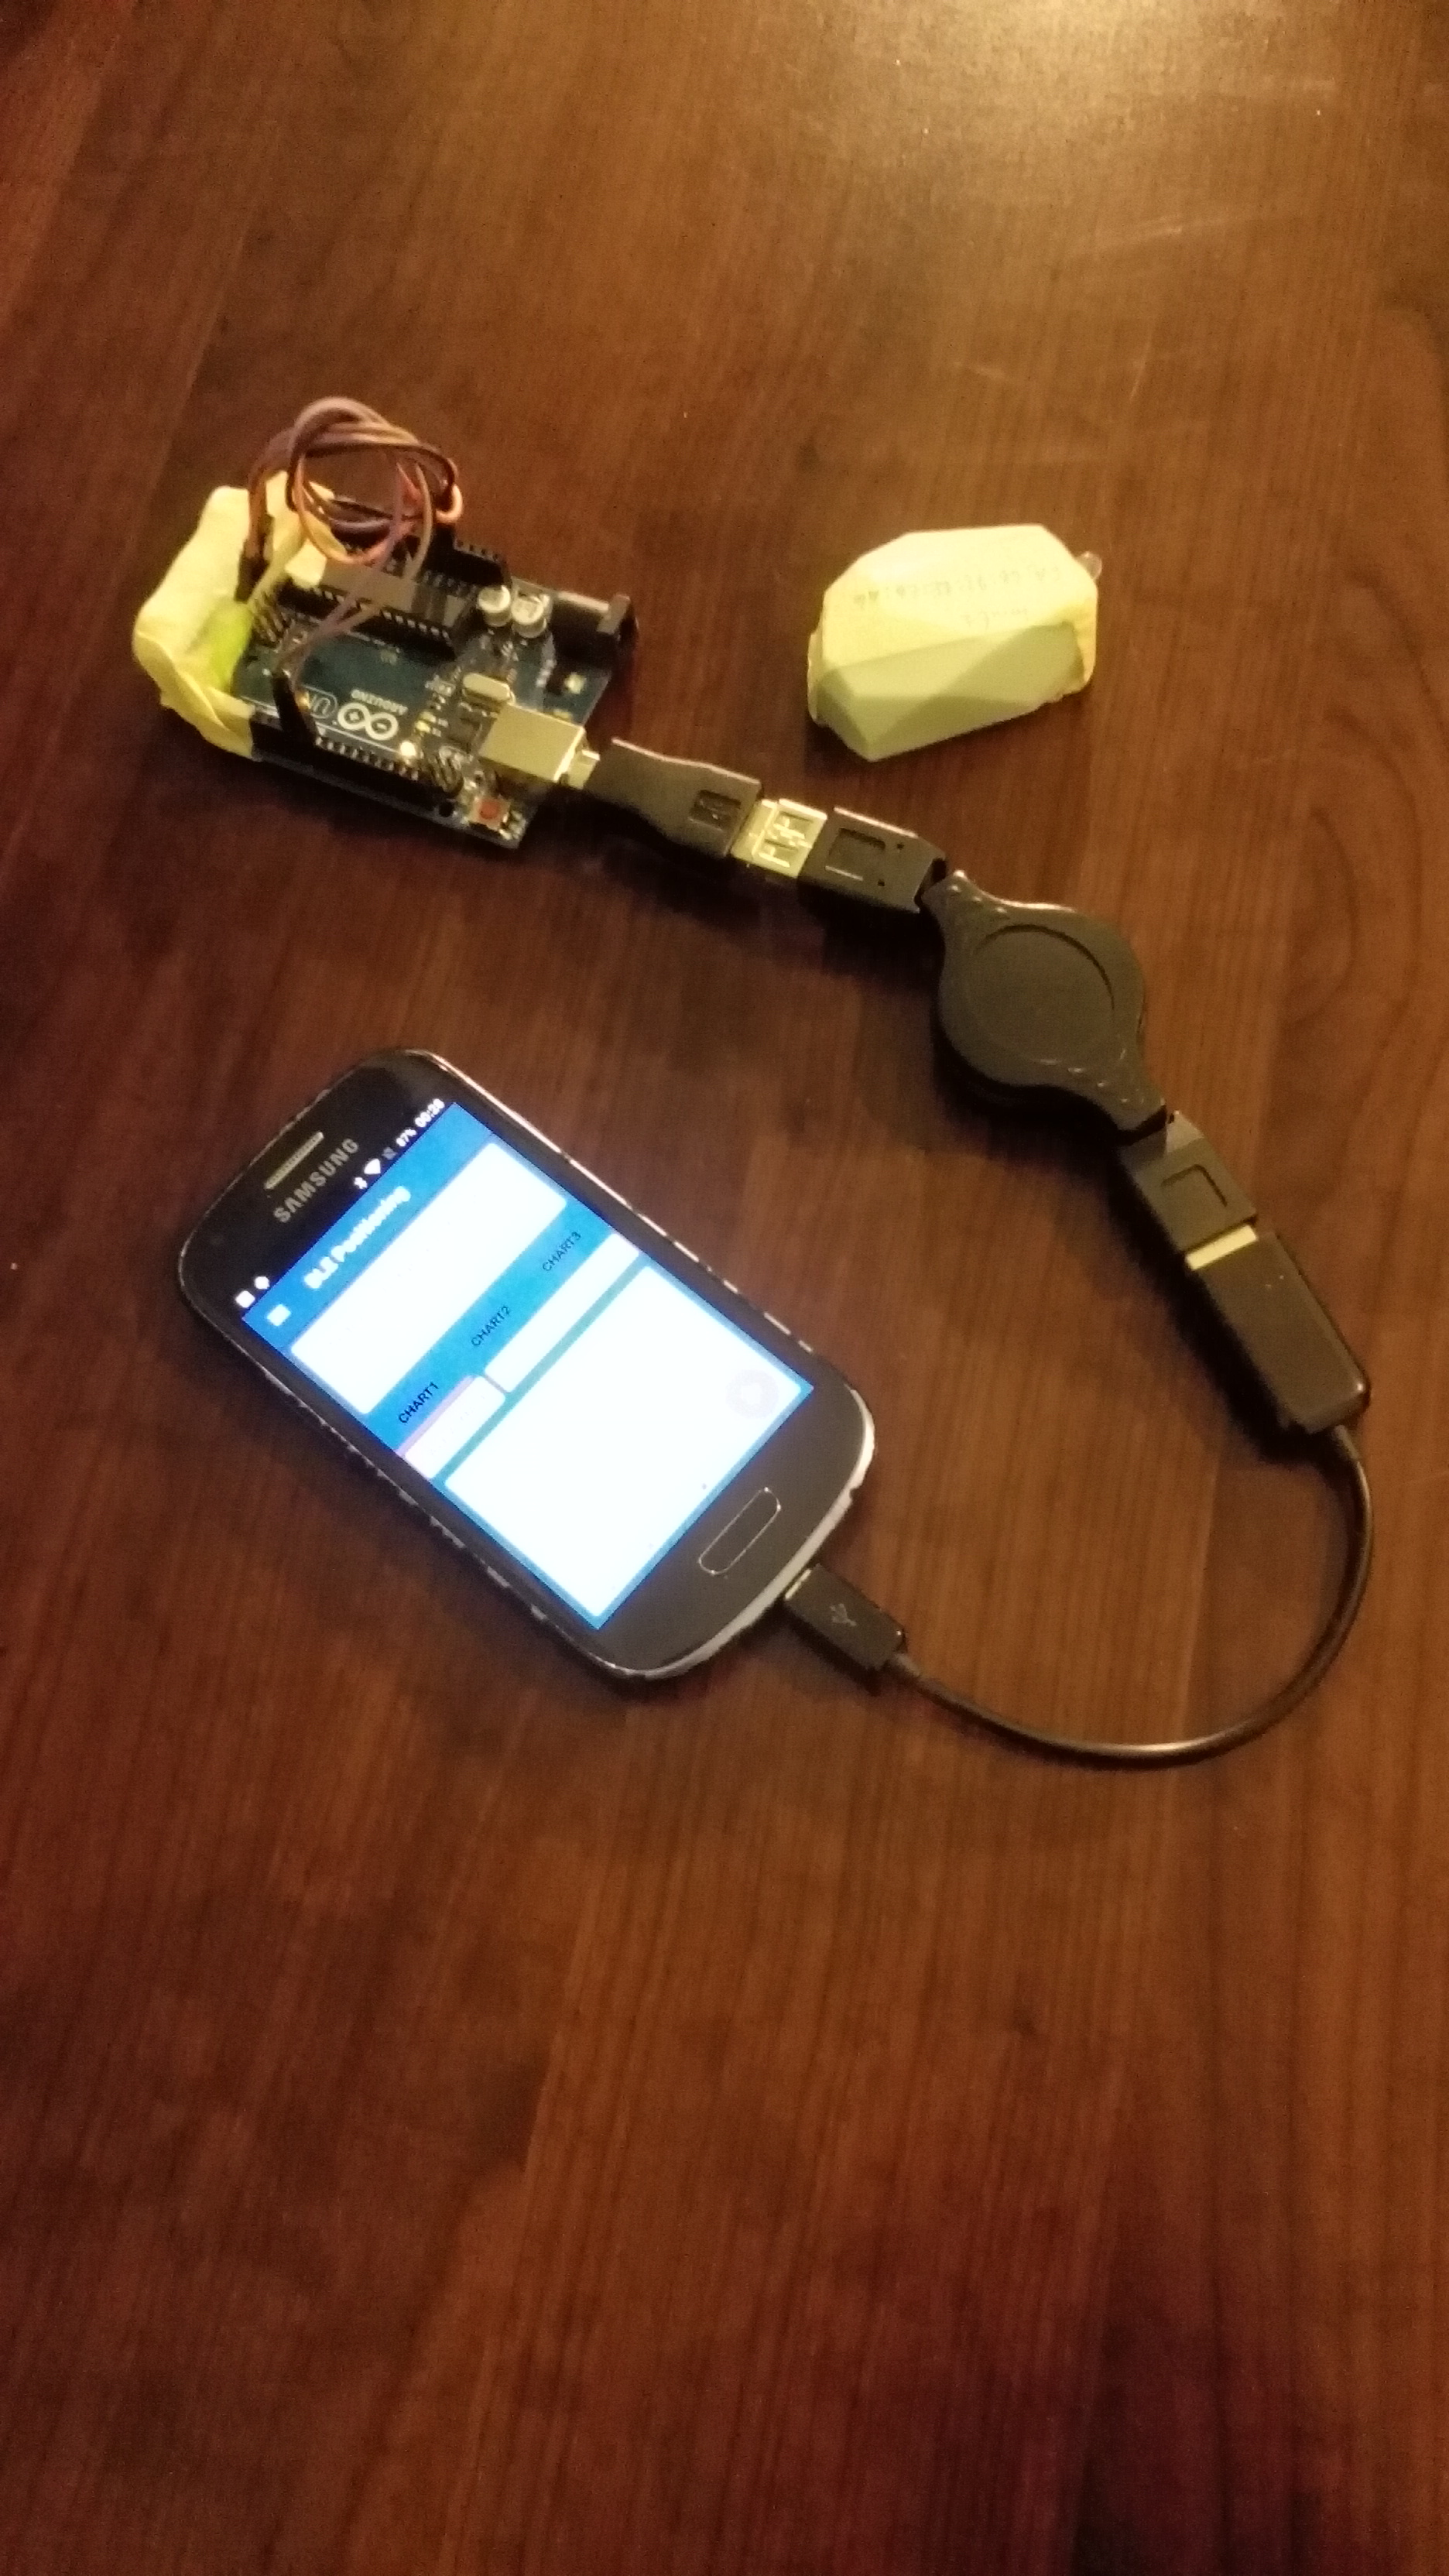
\includegraphics[width=0.3\linewidth]{img/otg/otg1.jpg}
	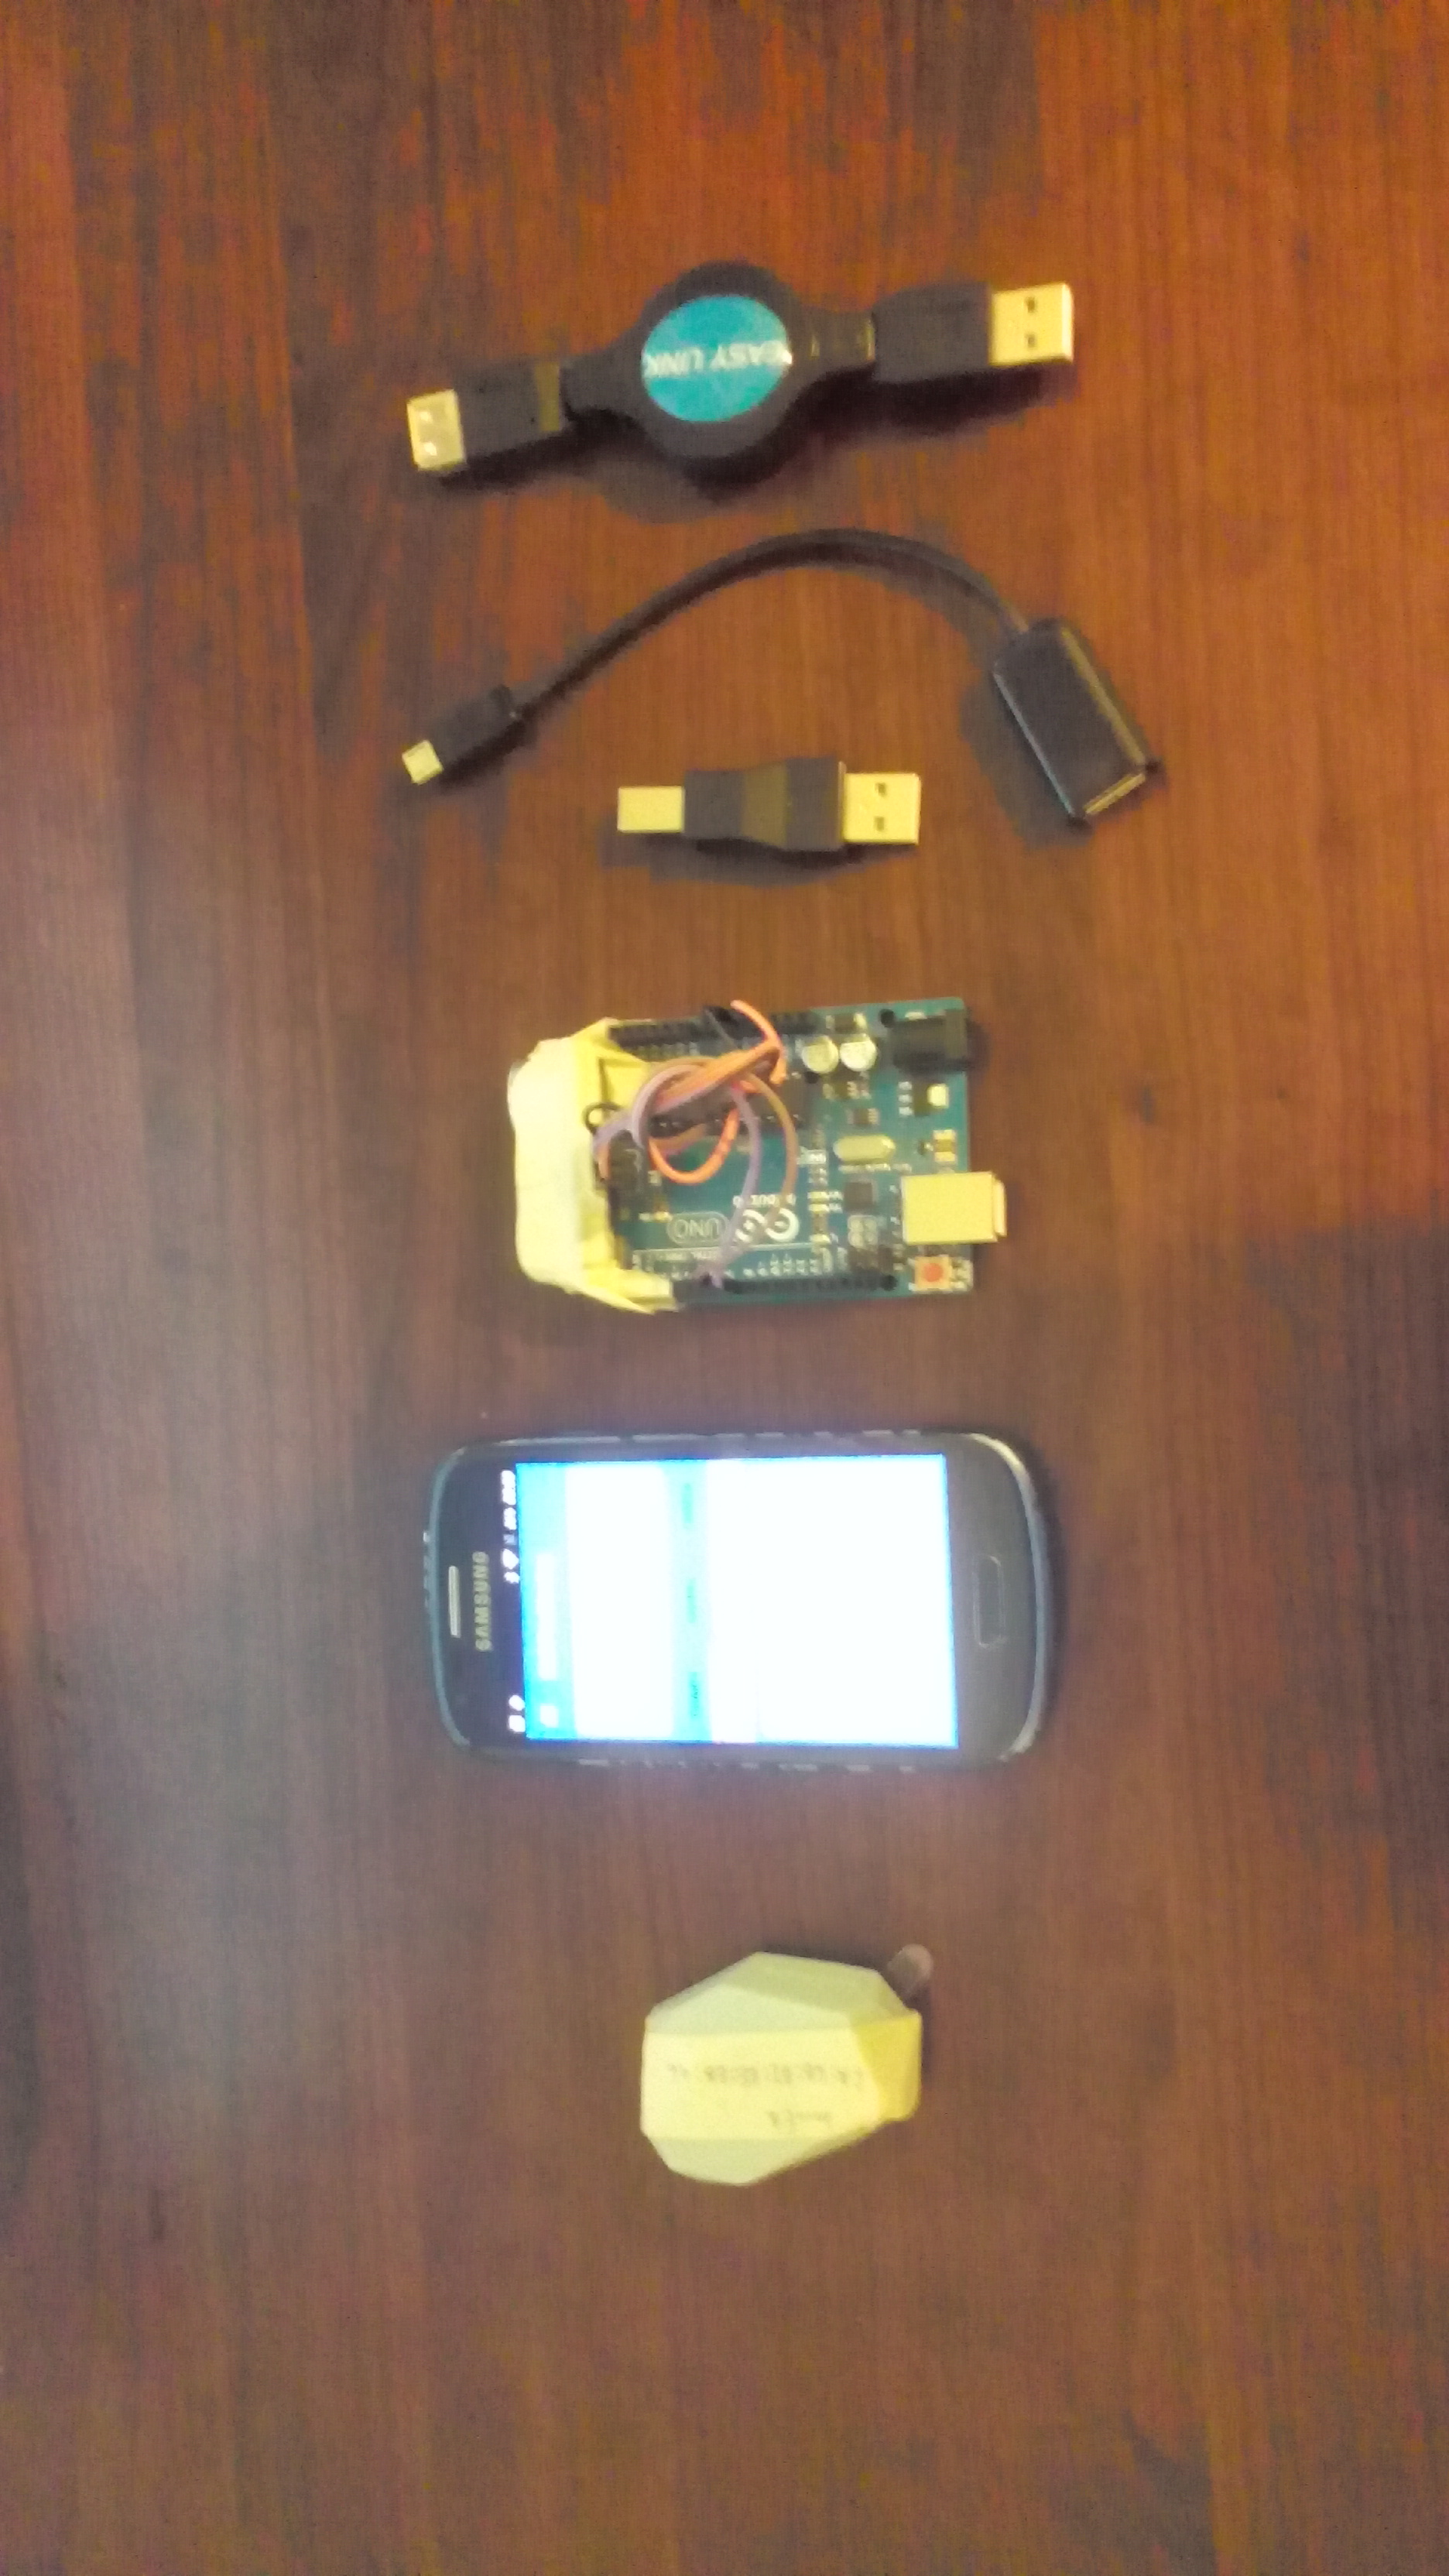
\includegraphics[width=0.3\linewidth]{img/otg/otg2.jpg}
	\caption{Collegamento Arduino-smartphone}
	\label{fig:collegamento_Arduino-smartphone}
\end{figure}

Questo approccio permette di avere un sensore di prossimità che restituisce una stima della distanza confrontabile con la stima eseguita con la tecnica RSSI.

\newpage
\subsection{Materiale utilizzato}
\begin{itemize}
	\item Samsung GT-I9190, \href{http://novafusion.pl/s3-mini/}{\textbf{CyanogenMod 12.1-20160718-UNOFFICIAL-golden Android 5.1.1}}\footnote{\href{http://novafusion.pl/s3-mini/}{\textbf{Novafusion}} - \url{http://novafusion.pl/s3-mini/}}.
	
	\item Sensore di prossimità ultrasonico HC-SR04.
	
	\item Cavo USB OTG ($ \sim 2$€).
	
\end{itemize}

\begin{figure}[ph]
	\centering
	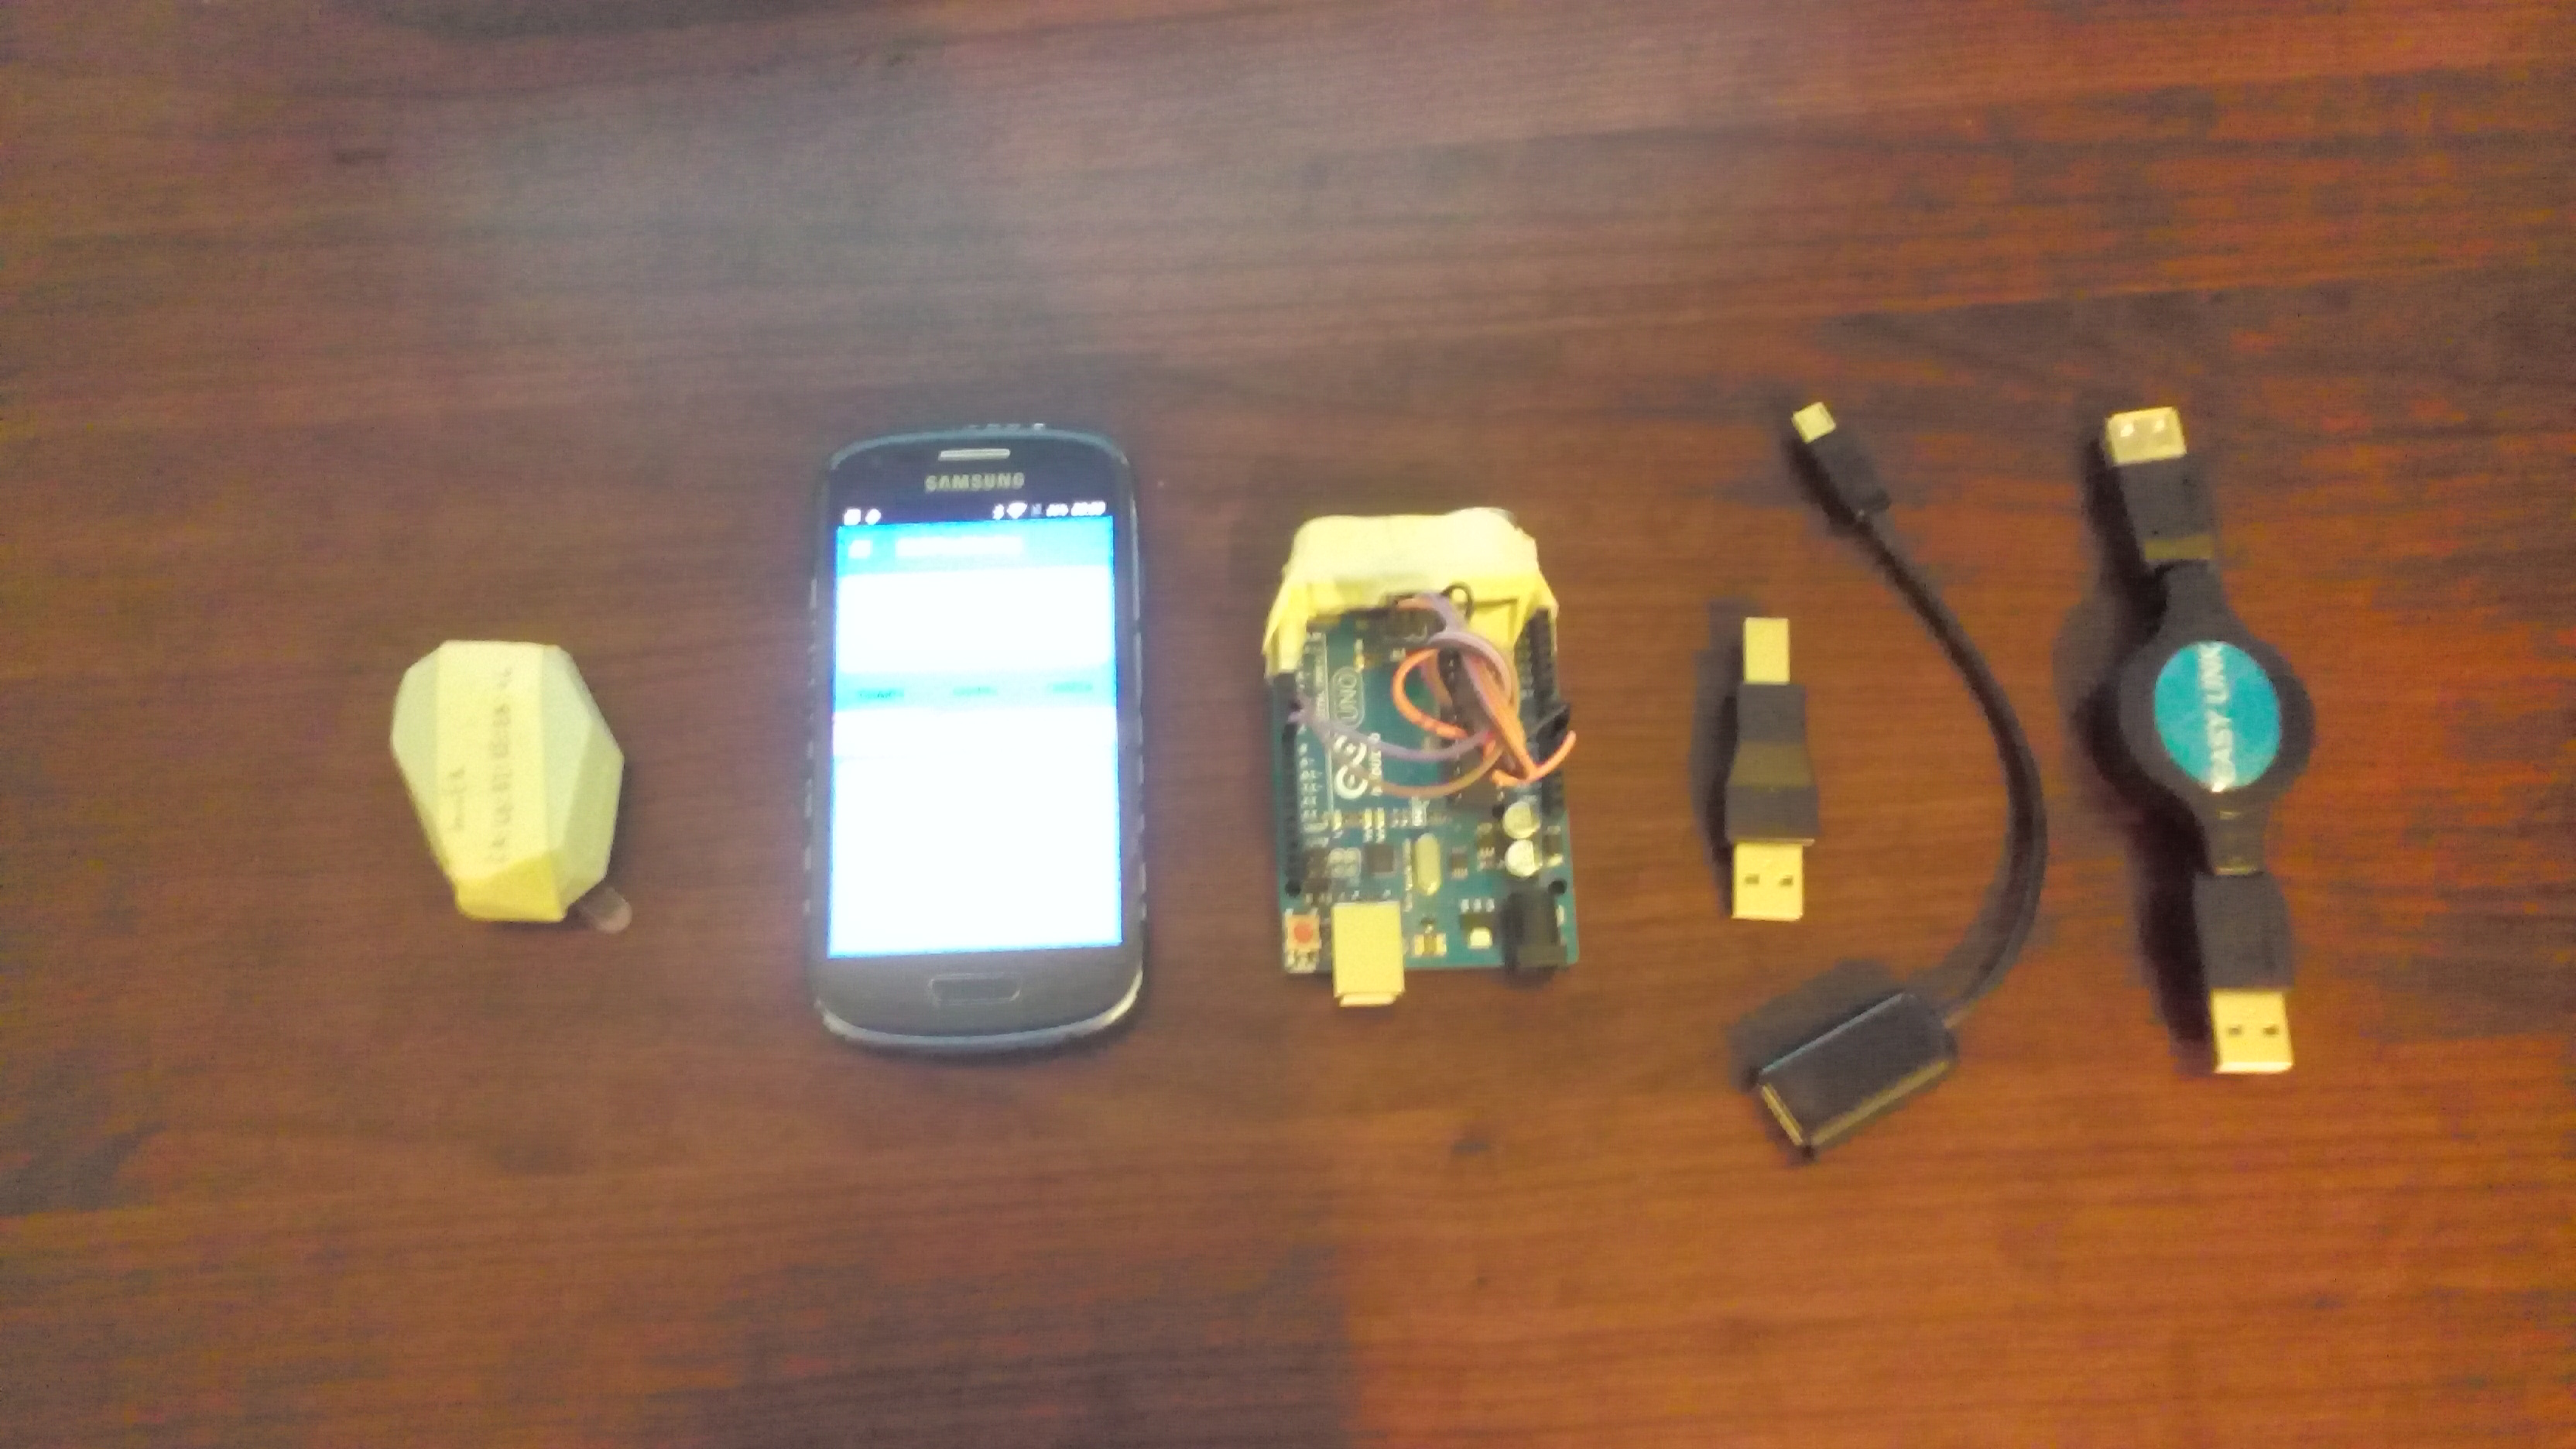
\includegraphics[width=0.8\linewidth]{img/otg/otg3.jpg}
	\caption{Materiale utilizzato}
\end{figure}

\newpage
\subsection{Dati raccolti}

\begin{tabular}{|c|c|c|}
	\hline 
	& Stima (m) & Deviazione (m) \\ 
	\hline 
	Min & 4,54 & +1.2m \\ 
	\hline 
	Max & 2 & 1 \\ 
	\hline 
	Avg & 2 & 3 \\ 
	\hline 
\end{tabular} 
